\subsection{Seiryu (清流)}
\vspace{-7mm}
\hspace{38mm}
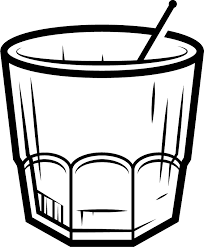
\includegraphics[width=4mm]{cocktail_glass_rock.png}
\vspace{2.5mm}
\begin{itembox}[l]{\boldmath $\reci$}
\begin{itemize}
\setlength{\parskip}{0cm}
\setlength{\itemsep}{0cm}
\item \sake 30ml
\item \bc 15ml
\item \lj 1tbsp
\item \limj 2tsp
\end{itemize}
\vspace{-4mm}
Made by \shake.
\end{itembox}
Seiryu means a clean stream. The light blue looks nice.
